\documentclass[tikz]{standalone}
% WIND / FORM -- an original Bauhaus-inspired interpretation of the source scene.
% Preserves the boy, tree, kite, and visible hand-to-kite connection.
% Flat primary colors, modular geometry, asymmetric balance, and negative space.
% Pure vector TikZ; no images, external fonts, gradients, or random dependencies.
% Compile: pdflatex -interaction=nonstopmode -halt-on-error -output-directory=tmp mweB.tex
% Upper-left coordinate origin; one drawing unit is one PDF big point.
\definecolor{paper}{HTML}{F2EBDD}
\definecolor{white}{HTML}{FFF9EE}
\definecolor{black}{HTML}{242528}
\definecolor{red}{HTML}{C84936}
\definecolor{yellow}{HTML}{E9B936}
\definecolor{blue}{HTML}{245995}
\definecolor{sand}{HTML}{DBCEB5}
\definecolor{skin}{HTML}{DDB58C}
\begin{document}
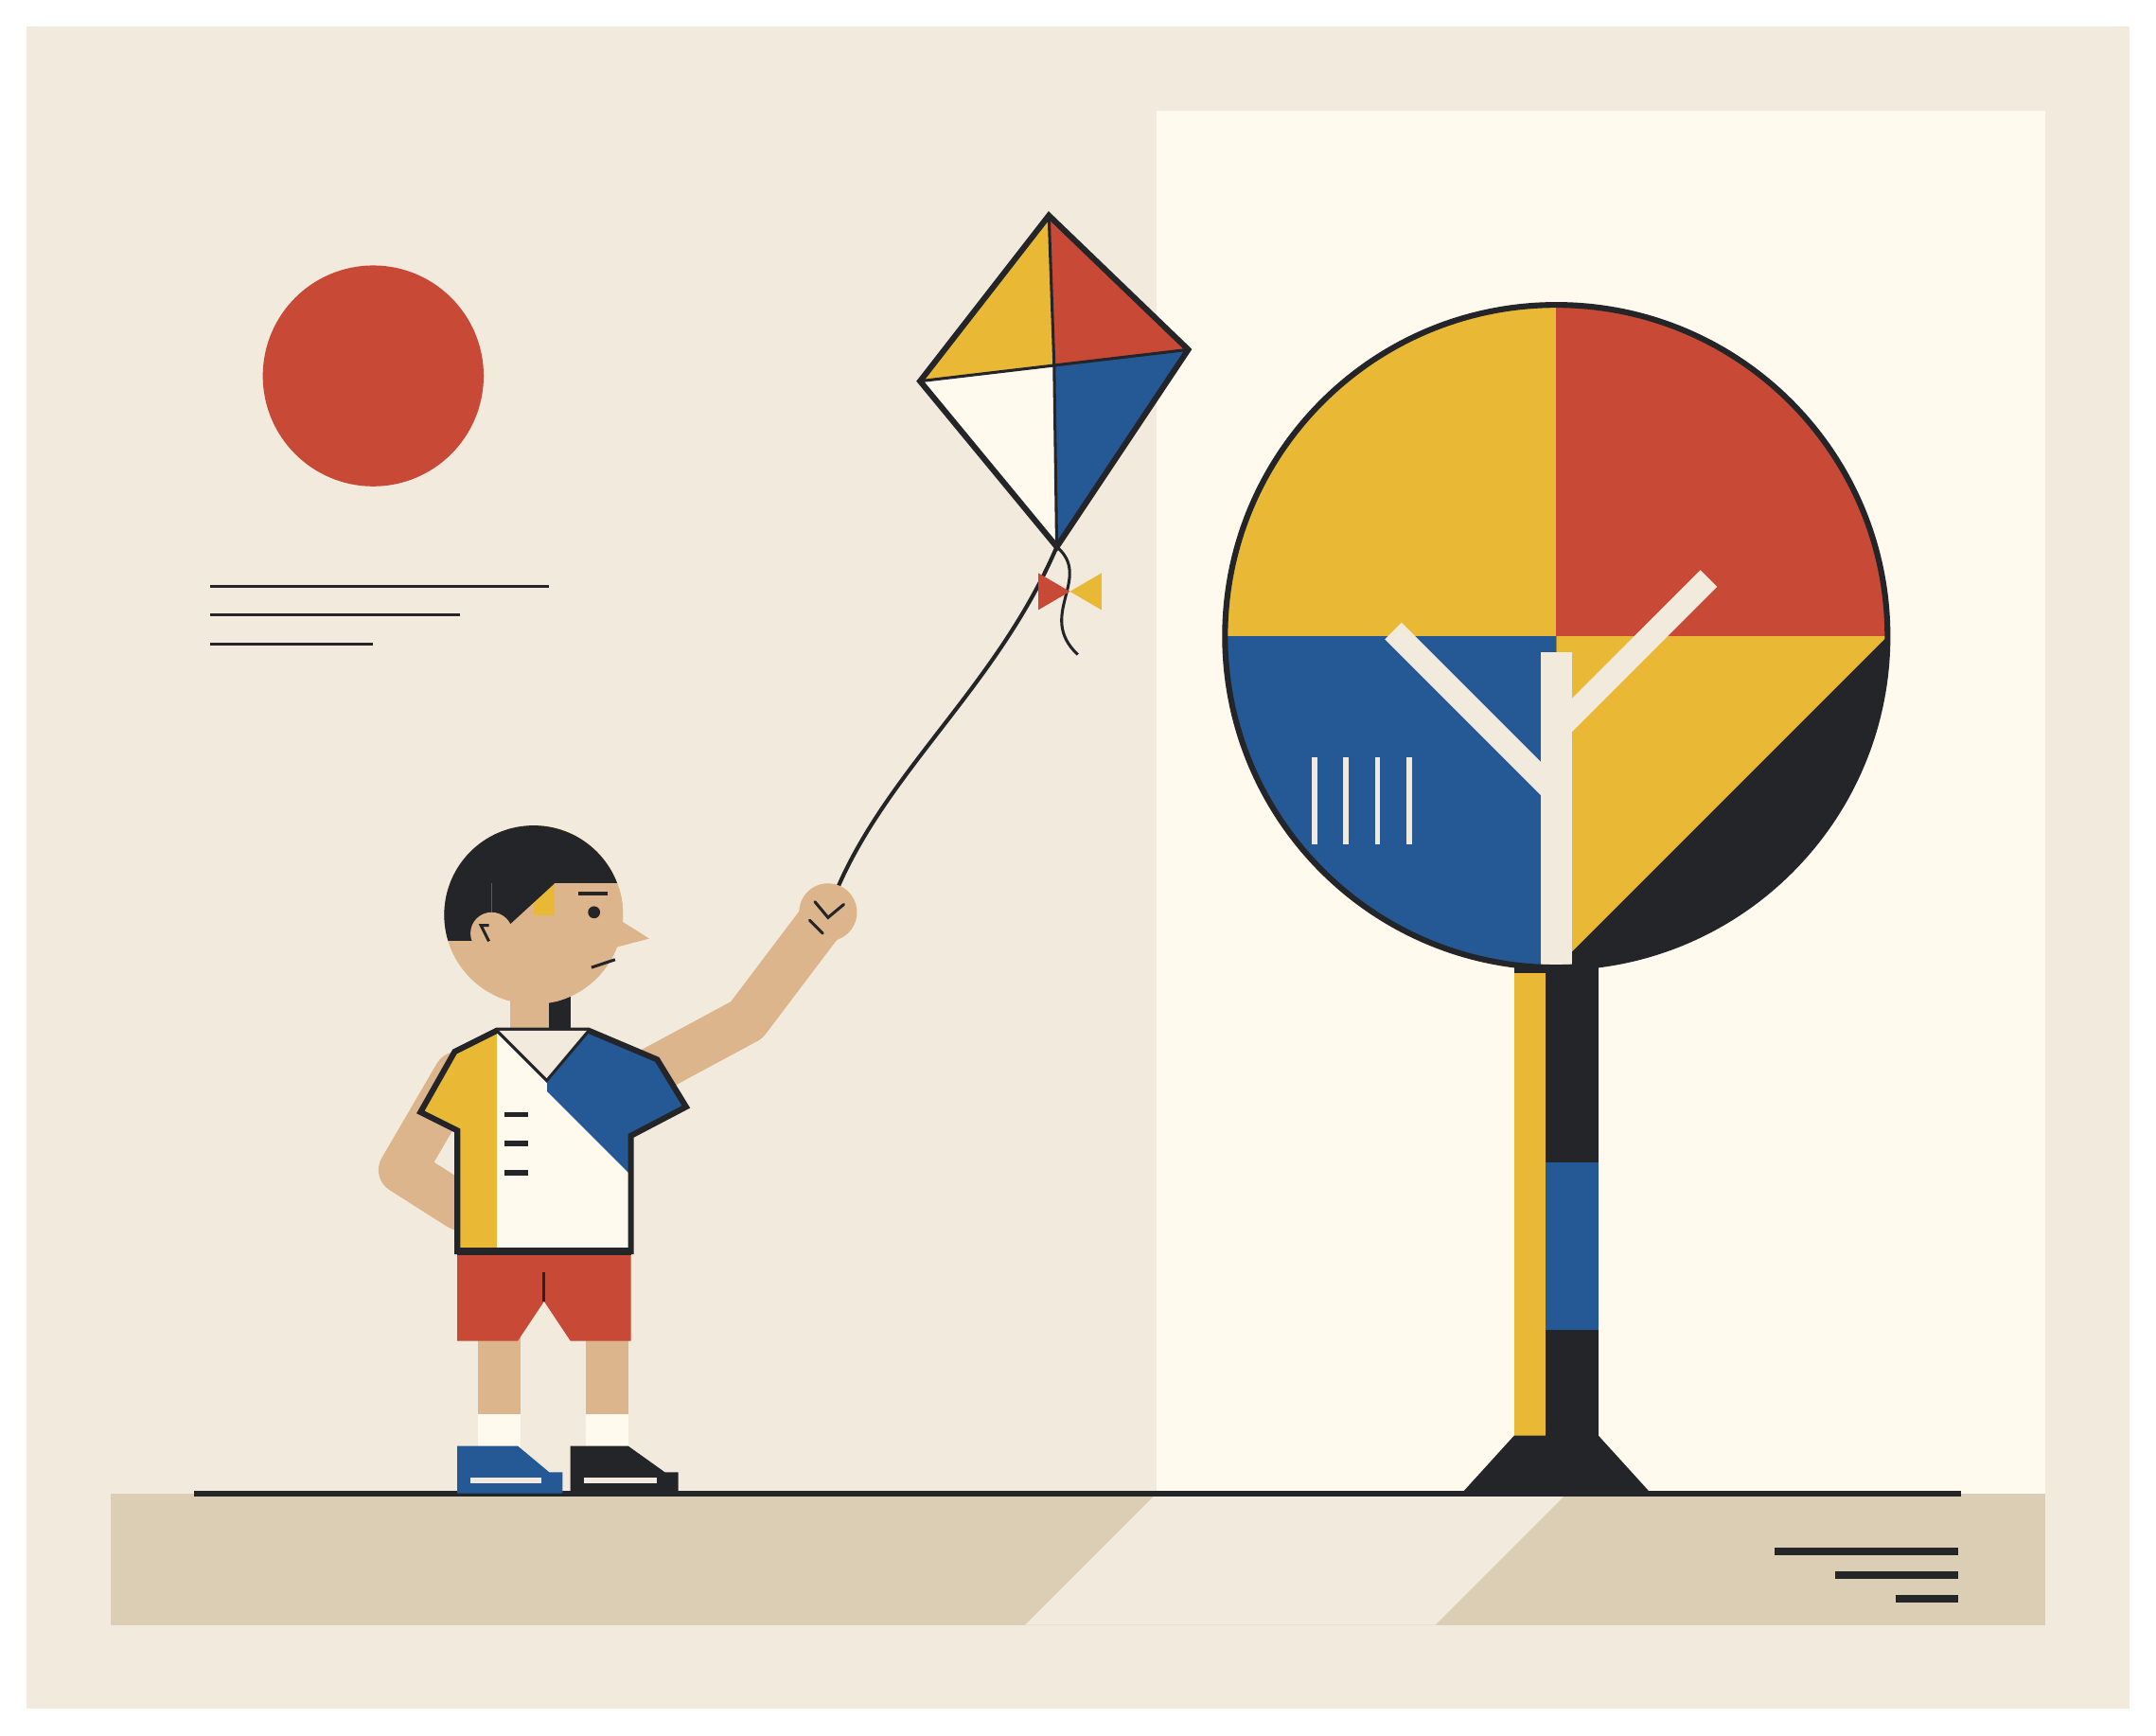
\begin{tikzpicture}[x=1bp,y=-1bp,line cap=butt,line join=miter,
  structure/.style={draw=black,line width=2.2bp},
  fine/.style={draw=black,line width=1.1bp},
  limb/.style={draw=skin,line width=18bp,line cap=round,line join=round}]
  \path[use as bounding box] (0,0) rectangle (800,640);
  \fill[paper] (0,0) rectangle (800,640);
  \begin{scope}
    \clip (32,32) rectangle (768,608);

    % 1. Quiet architectural field. A pale vertical plane anchors the tree.
    \fill[white] (430,32) rectangle (768,558);
    \fill[sand] (32,558) rectangle (768,608);
    \fill[paper] (430,558) -- (586,558) -- (536,608) -- (380,608) -- cycle;
    \draw[structure] (64,558) -- (736,558);
    % A restrained counterweight to the round crown, rather than a second subject.
    \fill[red] (132,133) circle[radius=42bp];
    \draw[fine] (70,213) -- (199,213);
    \draw[fine] (70,224) -- (165,224);
    \draw[fine] (70,235) -- (132,235);

    % 2. Tree: one circular crown, one trunk, two branches, one rooted base.
    \fill[black] (566,254) rectangle (598,558);
    \fill[yellow] (566,360) rectangle (578,543);
    \fill[blue] (578,432) rectangle (598,496);
    \fill[black] (566,536) -- (546,558) -- (618,558) -- (598,536) -- cycle;
    \coordinate (crown) at (582,232);
    \fill[yellow] (crown) circle[radius=126bp];
    \begin{scope}
      \clip (crown) circle[radius=126bp];
      % Orthogonal circle sectors express light and shade without modelling.
      \fill[blue] (456,232) rectangle (708,358);
      \fill[red] (582,106) rectangle (708,232);
      \fill[black] (582,232) rectangle (708,358);
      \fill[yellow] (582,232) -- (708,232) -- (582,358) -- cycle;
      % The branch motif is cut out in paper color, not another outline layer.
      \draw[draw=paper,line width=12bp] (582,368) -- (582,238);
      \draw[draw=paper,line width=9bp] (582,292) -- (520,230);
      \draw[draw=paper,line width=9bp] (582,268) -- (640,210);
      \foreach \x in {490,502,514,526}
        \draw[draw=paper,line width=2bp] (\x,278) -- (\x,311);
    \end{scope}
    % Only the crown perimeter gets an outline; the color seams stay flat.
    \draw[structure] (crown) circle[radius=126bp];

    % 3. Kite. Named anchors keep the spars, fabric, and string connected.
    \coordinate (kite-top) at (389,72);
    \coordinate (kite-right) at (442,123);
    \coordinate (kite-knot) at (392,198);
    \coordinate (kite-left) at (340,135);
    \coordinate (kite-center) at (391,129);
    \coordinate (hand) at (305,337);
    \draw[structure,line width=1.5bp] (hand)
      .. controls (323,286) and (368,254) .. (kite-knot);
    \fill[yellow] (kite-top) -- (kite-left) -- (kite-center) -- cycle;
    \fill[red] (kite-top) -- (kite-right) -- (kite-center) -- cycle;
    \fill[blue] (kite-right) -- (kite-knot) -- (kite-center) -- cycle;
    \fill[white] (kite-knot) -- (kite-left) -- (kite-center) -- cycle;
    \draw[structure] (kite-top) -- (kite-right) -- (kite-knot)
      -- (kite-left) -- cycle;
    \draw[fine] (kite-top) -- (kite-center) -- (kite-knot);
    \draw[fine] (kite-left) -- (kite-center) -- (kite-right);
    \draw[fine] (kite-knot) .. controls (406,210) and (384,224) .. (400,239);
    \fill[red] (397,215) -- (385,208) -- (385,222) -- cycle;
    \fill[yellow] (397,215) -- (409,208) -- (409,222) -- cycle;

    % 4. Boy: elementary shapes retain a readable human gesture and profile.
    % Legs, socks, and shoes use the same modular widths.
    \fill[skin] (172,488) rectangle (188,545);
    \fill[skin] (213,488) rectangle (229,545);
    \fill[white] (172,528) rectangle (188,545);
    \fill[white] (213,528) rectangle (229,545);
    \fill[blue] (164,540) -- (187,540) -- (199,550)
      -- (204,550) -- (204,558) -- (164,558) -- cycle;
    \fill[black] (207,540) -- (229,540) -- (243,550)
      -- (248,550) -- (248,558) -- (207,558) -- cycle;
    \draw[draw=paper,line width=2bp] (169,553) -- (196,553);
    \draw[draw=paper,line width=2bp] (212,553) -- (240,553);

    % Bent arm and raised forearm: round joints soften the rectangular torso.
    \draw[limb] (164,399) -- (143,435) -- (165,449);
    \draw[limb] (235,399) -- (274,378) -- (hand);
    \fill[skin] (hand) circle[radius=11bp];
    \draw[fine,line cap=round] (300,333) -- (305,339) -- (311,334);
    \draw[fine,line cap=round] (298,340) -- (303,345);
    \fill[black] (184,354) rectangle (207,390);
    \fill[skin] (184,354) rectangle (199,390);

    % Shirt: one silhouette and clipped primary-color modules.
    \def\Shirt{(179,382) -- (214,382) -- (240,393) -- (251,411)
      -- (230,422) -- (230,466) -- (164,466) -- (164,420)
      -- (150,413) -- (163,390) -- cycle}
    \path[fill=white] \Shirt;
    \begin{scope}
      \clip \Shirt;
      \fill[blue] (198,382) rectangle (251,466);
      \fill[yellow] (150,382) rectangle (179,466);
      \fill[white] (198,405) -- (230,437) -- (230,466) -- (198,466) -- cycle;
      \draw[draw=black,line width=2bp] (182,414) -- (191,414);
      \draw[draw=black,line width=2bp] (182,425) -- (191,425);
      \draw[draw=black,line width=2bp] (182,436) -- (191,436);
    \end{scope}
    \draw[structure] \Shirt;
    \path[fill=paper] (179,382) -- (198,401) -- (214,382) -- cycle;
    \draw[fine] (179,382) -- (198,401) -- (214,382);

    % The original red shorts remain a strong identifying color cue.
    \fill[red] (164,466) -- (230,466) -- (230,500)
      -- (207,500) -- (197,485) -- (187,500) -- (164,500) -- cycle;
    \draw[draw=black,line width=3bp] (164,466) -- (230,466);
    \draw[fine] (197,485) -- (197,474);

    % Circular head with a semicircular hair cap, triangular nose, and one eye.
    \coordinate (head) at (193,338);
    \fill[skin] (head) circle[radius=34bp];
    \fill[skin] (218,335) -- (237,347) -- (218,352) -- cycle;
    \begin{scope}
      \clip (head) circle[radius=34bp];
      \fill[yellow] (193,304) rectangle (227,338);
      \fill[skin] (201,325) rectangle (232,373);
      \fill[black] (159,304) rectangle (227,326);
      \fill[black] (159,326) rectangle (177,348);
      \fill[black] (177,326) -- (201,326) -- (177,348) -- cycle;
    \end{scope}
    \fill[skin] (177,345) circle[radius=8bp];
    \draw[fine] (176,342) -- (173,342) -- (176,348);
    \fill[black] (216,337) circle[radius=2.3bp];
    \draw[draw=black,line width=1.5bp] (210,330) -- (221,330);
    \draw[fine] (215,358) -- (224,355);

    % Three ground bars echo the upper-left rhythm, with no textual labels.
    \draw[draw=black,line width=3bp] (665,580) -- (735,580);
    \draw[draw=black,line width=3bp] (688,589) -- (735,589);
    \draw[draw=black,line width=3bp] (711,598) -- (735,598);
  \end{scope}
\end{tikzpicture}
\end{document}
